
\chapter{Exploratory Data Analysis}\label{app:exploratory_data_analysis}

This appendix presents the exploratory data analysis of the two regional datasets. The analyses were conducted prior to model development and informed several key methodological decisions: the choice of linear detrending, the inclusion of previous-year (y0) features, the identification of likely era-confounded variables, and the feature selection strategy for CarenR. All statistics are computed from the final curated datasets (dataPrep\_cont\_dataset\_rdd.csv and dataPrep\_cont\_dataset\_rvv.csv) unless otherwise noted.


\section{Wine Production: Descriptive Statistics and Trends}\label{app_sec:wine_production_descriptive_statistics}

Table~\ref{tab:appb_1} presents the key descriptive statistics for wine production in both regions over the full study period.

\begin{table}[htbp]
  \centering
  \caption{Descriptive statistics: RDD (1934--2022) and RVV (1942--2021).}\label{tab:appb_1}
  \footnotesize
  \begin{adjustbox}{max width=\textwidth}
    \begin{tabularx}{\textwidth}{l|l|X}
  \toprule
  Statistic & RDD (Douro)
1934--2022 & RVV (Vinho Verde)
1942--2021 \\
  \midrule
  Observations (n) & 89 years & 80 years \\
  Mean production & 1,116 mhl & 1,621 mhl \\
  Standard deviation & 307 mhl & 751 mhl \\
  Coefficient of variation (CV) & 27.6\% & 46.4\% \\
  Minimum & 518 mhl (1952) & 494 mhl (1997) \\
  Maximum & 1,961 mhl (1990) & 3,443 mhl (1962) \\
  Linear trend slope & +7.4 mhl/year (increasing) & $-$21.2 mhl/year (declining) \\
  Total change over period & +~660 mhl (~+80\%) & $-$~1,500 mhl (~$-$65\%) \\
  \bottomrule
  \end{tabularx}
  \end{adjustbox}

\end{table}


The contrast between the two regions is immediately apparent. Vinho Verde has a substantially higher mean production (1,621 vs 1,116 mhl) and nearly three times the standard deviation (751 vs 307 mhl), yielding a CV of 46.4\% vs 27.6\%. This higher variability in RVV is partly structural, the larger absolute production values amplify variation, but also reflects the stronger era-driven structural changes in the RVV series. The coefficient of variation is a key number for understanding the prediction task: with CV = 27.6\% for RDD and 46.4\% for RVV, any model must reduce the residual error substantially below the naive prediction to be useful, which is a high bar with a climate signal explaining only ~22\% of variance.


\subsection{Decade-Level Production Averages}\label{app_sub:decadelevel_production_averages}

Table~\ref{tab:appb_2} presents decade-level mean production for both regions, revealing the structural trajectory of each series.

\begin{table}[htbp]
  \centering
  \caption{Decade-level production averages for RDD and RVV.}\label{tab:appb_2}
  \footnotesize
  \begin{adjustbox}{max width=\textwidth}
    \begin{tabularx}{\textwidth}{l|p{4.5cm}|l|l|X}
  \toprule
  Decade & RDD mean (mhl) & RDD n & RVV mean (mhl) & RVV n \\
  \midrule
  1930s & 765 & 7 & --- & --- \\
  1940s & 767 & 10 & 2,026 & 9 \\
  1950s & 926 & 10 & 1,941 & 10 \\
  1960s & 1,184 & 10 & 2,331 & 10 \\
  1970s & 1,090 & 10 & 2,229 & 10 \\
  1980s & 1,148 & 10 & 1,638 & 10 \\
  1990s & 1,271 & 10 & 1,259 & 10 \\
  2000s & 1,392 & 10 & 906 & 10 \\
  2010s & 1,308 & 10 & 798 & 10 \\
  2020s & 1,287 & 3 & 871 & 2 \\
  \bottomrule
  \end{tabularx}
  \end{adjustbox}

\end{table}


The decade table makes the structural stories of both regions clearly visible. RDD production roughly doubled between the 1930s--40s (765--767 mhl) and the 2000s--2010s (1,300--1,400 mhl), with the most rapid growth occurring in the 1950s--60s and again in the 1990s--2000s. The slowdown in the 2010s is consistent with the maturation of the Douro DOC expansion and the administrative constraints of the Port benef\'icio quota system. For RVV, the peak decade was the 1960s (2,331 mhl), with a sharp decline beginning in the 1980s (1,638 mhl), continuing steeply into the 2000s (906 mhl), exactly coinciding with Portugal's EU accession (1986) and the structural reforms that followed. By the 2010s, RVV production had fallen to approximately one-third of its 1960s peak.

These structural trajectories directly explain the era confound described throughout the thesis. In both regions, the linear trend does not fully capture the non-linear shape of the production history, particularly the RVV plateau in the 1970s (2,229 mhl, barely below the 1960s peak) followed by a sharp break in the 1980s. This structural break is the primary reason LOESS detrending performs better than linear detrending for RVV (Section~\ref{sec:detrend_sensitivity_analysis_loess}): the flexible LOESS curve can fit the plateau-then-collapse shape, while the linear trend averages over it, leaving systematic residuals in the 1970s.


\section{Phenological Timing: Trends and Variability}\label{app_sec:phenological_timing_trends_and}

The phenological dates used as anchors for feature engineering are themselves variable across years and show systematic advancement over the study period, consistent with the warming trends documented in the broader viticulture literature. Table~\ref{tab:appb_3} summarises the mean, variability, and long-term trend for each key phenological stage. Negative trends indicate earlier occurrence over time; all trends are expressed in days per decade.

\begin{table}[htbp]
  \centering
  \caption{Phenological timing: mean dates, variability, and decadal trends.}\label{tab:appb_3}
  \footnotesize
  \begin{adjustbox}{max width=\textwidth}
    \begin{tabularx}{\textwidth}{p{2.2cm}|p{2cm}|p{1.4cm}|p{1.9cm}|p{2cm}|p{1.4cm}|X}
  \toprule
  Stage & RDD mean
(DOY / date) & RDD SD
(days) & RDD trend
(days/decade) & RVV mean
(DOY / date) & RVV SD
(days) & RVV trend
(days/decade) \\
  \midrule
  Bud Break (BB) & DOY 88 / 27 Mar & 8.4 & $-$0.5 & DOY 90 / 30 Mar & 9.2 & $-$1.0 \\
  Flowering (Fl) & DOY 135 / 14 May & 9.8 & $-$0.7 & DOY 154 / 2 Jun & 12.0 & $-$1.1 \\
  Start Maturity (sM) & DOY 179 / 27 Jun & 8.6 & $-$0.9 & DOY 227 / 14 Aug & 13.6 & $-$1.7 \\
  Harvest (Hv) & DOY 257 / 13 Sep & 13.3 & $-$1.9 & DOY 270 / 26 Sep & 17.0 & $-$2.6 \\
  \bottomrule
  \end{tabularx}
  \end{adjustbox}

\end{table}


Several findings stand out. First, harvest timing is advancing most rapidly in both regions, by approximately 1.9 days per decade in RDD and 2.6 days per decade in RVV. Over the 80--90 year study period this represents an advancement of roughly 15--23 days, consistent with the warming of 1.3$^\circ$C in growing-season temperature projected and partly already observed in Portuguese wine regions \citep{Cunha2016}. Earlier harvest is a well-documented consequence of warming: grapes accumulate heat units faster, reaching physiological maturity sooner. Second, the trend is stronger in RVV than in RDD for every stage, which is consistent with the Atlantic climate's stronger sensitivity to warming, in a wetter regime, higher temperatures have a disproportionate effect on evapotranspiration and vine water status, accelerating phenological development.

Second, the variability (SD) in phenological dates is larger in RVV than RDD for all stages, particularly for start of maturity (13.6 vs 8.6 days) and harvest (17.0 vs 13.3 days). This higher phenological variability in RVV is consistent with the region's more variable Atlantic weather: ocean-driven temperature swings create larger year-to-year variation in the timing of heat accumulation. This greater phenological variability also means that fixed-calendar aggregation windows would be a poor substitute for the phenological-anchor approach used in this thesis: a fixed "September temperature" window would capture completely different vine developmental states in an early harvest year vs a late harvest year.


\subsection{Growing Season Duration}\label{app_sub:growing_season_duration}

Table~\ref{tab:appb_4} shows the mean duration of each inter-stage phase for both regions.

\begin{table}[htbp]
  \centering
  \caption{Production statistics by era for RDD and RVV.}\label{tab:appb_4}
  \footnotesize
  \begin{adjustbox}{max width=\textwidth}
    \begin{tabularx}{\textwidth}{p{2.0cm}|p{2.2cm}|p{1.5cm}|p{1.8cm}|p{1.5cm}|X}
  \toprule
  Phase & RDD mean & RDD SD & RVV mean & RVV SD & Interpretation \\
  \midrule
  Budburst $\rightarrow$ Flowering & 47.0 days & 7.9d & 64.3 days & 9.0d & RVV flowering 17d later than RDD on average, cooler Atlantic spring \\
  Flowering $\rightarrow$ Veraison & 44.8 days & 4.9d & 73.0 days & 6.9d & RVV takes 28d longer to reach veraison, slower ripening in Atlantic climate \\
  Veraison $\rightarrow$ Harvest & 78.1 days & 6.5d & 42.7 days & 7.7d & RDD takes longer from veraison to harvest, slower final ripening phase \\
  Full season (BB$\rightarrow$Hv) & 169.9 days & 12.6d & 180.0 days & 13.8d & RVV growing season ~10 days longer overall \\
  \bottomrule
  \end{tabularx}
  \end{adjustbox}

\end{table}


The phase durations reveal important differences in growing season structure. The flowering-to-veraison phase is 28 days longer in RVV (73 vs 45 days), the Atlantic climate's slower heat accumulation extends this key berry development phase. Conversely, the veraison-to-harvest phase is substantially longer in RDD (78 vs 43 days), reflecting that Douro grapes undergo a longer slow-ripening phase under the drier semi-arid conditions before reaching harvest maturity. These structural differences mean that features from the same phenological window cover different absolute calendar periods in the two regions, and directly motivate the use of separate feature construction and model fitting for each region rather than a pooled approach.


\section{Feature Correlations with Production}\label{app_sec:feature_correlations_with_production}

Table~\ref{tab:appb_5} shows the ten features most strongly correlated with wine production residuals (detrended) in each region. This analysis was part of the exploratory phase that informed the feature selection strategies evaluated in CarenR. In the direction column, + indicates positive correlation with production and $-$ negative.

\begin{table}[htbp]
  \centering
  \caption{Feature correlations with detrended production ($|r|$) for RDD and RVV.}\label{tab:appb_5}
  \footnotesize
  \begin{adjustbox}{max width=\textwidth}
    \begin{tabularx}{\textwidth}{l|p{3.4cm}|p{1.3cm}|p{1.5cm}|p{3.4cm}|p{1.3cm}|X}
  \toprule
  Rank & RDD feature & RDD |r| & Direction & RVV feature & RVV |r| & Direction \\
  \midrule
  1 & tm\_hv\_y1\_c10
(harvest temp) & 0.386 & + & iaf\_hv\_y1\_c10
(LAI at harvest) & 0.404 & $-$ \\
  2 & tn\_hv\_y0\_a30
(prev-yr harvest nights) & 0.347 & + & tm\_hv\_y1\_b20
(pre-harvest temp) & 0.402 & $-$ \\
  3 & swa\_fl\_y1\_a30
(post-fl soil water) & 0.283 & $-$ & tm\_sm\_y1\_c20
(maturity temp) & 0.342 & $-$ \\
  4 & iaf\_fl\_y0\_b20
(prev-yr fl LAI) & 0.276 & $-$ & tn\_hv\_y0\_a30
(prev-yr harvest nights) & 0.325 & $-$ \\
  5 & iaf\_fl\_y0\_b30
(prev-yr fl LAI, wide) & 0.268 & $-$ & days.rf.above.1mm\_fl\_y1\_a20
(wet days post-fl) & 0.306 & $-$ \\
  6 & swa\_fl\_y1\_a15
(post-fl soil water) & 0.261 & $-$ & tm\_sm\_y0\_a20
(prev-yr summer temp) & 0.302 & $-$ \\
  7 & tm\_hv\_y1\_b20
(pre-harvest temp) & 0.248 & + & rf\_fl\_y1\_a10
(post-fl rainfall) & 0.288 & $-$ \\
  8 & tm.days.less.15\_fl\_y1\_b15
(cold days at fl) & 0.245 & $-$ & days.rf.above.1mm\_fl\_y1\_c15
(wet days at fl) & 0.264 & $-$ \\
  9 & iaf\_fl\_y0\_b10
(prev-yr fl LAI) & 0.227 & $-$ & tm\_hv\_y1\_c10
(harvest temp) & 0.253 & $-$ \\
  10 & swa\_hv\_y1\_b20
(harvest soil water) & 0.223 & $-$ & swa\_hv\_y1\_b20
(harvest soil water) & 0.245 & + \\
  \bottomrule
  \end{tabularx}
  \end{adjustbox}

\end{table}


Several observations from this correlation table are noteworthy. First, swa\_hv\_y1\_b20 (harvest soil water) appears in the top 10 for both regions, but with opposite signs, negative (r = $-$0.223) for RDD and positive (r = +0.245) for RVV. This is the same directional inversion identified in the CarenR rules (Section~\ref{sub:the_directional_inversion_a}), now confirmed at the simple correlation level. Second, the top RDD correlate is harvest temperature (r = +0.386), which does not prominently appear in the top CarenR rules because CarenR uses discretised variables and the KS test detects distributional shift rather than linear correlation. The harvest temperature signal is captured by M5Rules (positive coefficients) and RIPPER (harvest temperature in Rules 1--2) instead. Third, the top RVV correlate is LAI at harvest (r = $-$0.404), consistent with its dominance in the CarenR RVV rule set. The negative sign confirms that higher LAI reduces production, the canopy vigour mechanism discussed throughout Chapter~\ref{ch:goal_1_rule_extraction}.


\section{Feature Drift: The Era Confound Quantified}\label{app_sec:feature_drift_the_era}

A critical question for interpreting the CarenR rules is which features are genuinely informative about inter-annual climate variation and which are primarily capturing the long-term structural trend (era membership). Features strongly correlated with calendar year are suspected era-confounders: they co-vary with the production trend for structural reasons rather than because they drive production through a climate mechanism. Table~\ref{tab:appb_6} shows the features most strongly correlated with year for both regions; features marked HIGH co-trend strongly with the production structural trend.

\begin{table}[htbp]
  \centering
  \caption{Feature drift: correlation with year index as proxy for era confound.}\label{tab:appb_6}
  \footnotesize
  \begin{adjustbox}{max width=\textwidth}
    \begin{tabularx}{\textwidth}{l|p{2.6cm}|p{1.5cm}|p{2.3cm}|p{2.6cm}|p{1.5cm}|X}
  \toprule
  Rank & RDD feature & r(feat, year) & Concern level & RVV feature & r(feat, year) & Concern level \\
  \midrule
  1 & tm\_hv\_y1\_c10
(harvest temp) & +0.412 & HIGH, warming trend & tm\_sm\_y1\_c20
(maturity temp) & +0.402 & HIGH, warming trend \\
  2 & tm\_hv\_y1\_b20
(pre-harvest temp) & +0.373 & HIGH & iaf\_hv\_y1\_c10
(LAI at harvest) & +0.359 & MODERATE \\
  3 & tn\_hv\_y0\_a30
(prev-yr harvest nights) & +0.371 & HIGH, warming & tm\_sm\_y0\_b20
(prev-yr maturity temp) & +0.348 & HIGH \\
  4 & tm\_sm\_y0\_a20
(prev-yr summer temp) & +0.269 & MODERATE & tm\_hv\_y1\_b20
(pre-harvest temp) & +0.335 & HIGH \\
  5 & days.rf.above.1mm\_hv
(harvest rain days) & $-$0.201 & LOW & tm\_sm\_y0\_a20
(prev-yr summer temp) & +0.295 & MODERATE \\
  \bottomrule
  \end{tabularx}
  \end{adjustbox}

\end{table}


The harvest temperature variable (tm\_hv\_y1\_c10) is the most era-confounded feature in the dataset: it correlates with production at r = +0.386 (RDD) but also correlates with year at r = +0.412. This near-equal correlation with both production and time is a warning sign: the feature may appear predictive of production largely because both are trending upward over the study period (warming climate + increasing Douro production), rather than because harvest temperature genuinely drives production inter-annually. The LOESS validation (Section~\ref{sec:loess_validation_distinguishing_signal}) addresses this precisely: after removing the era trend, the top features'  correlations drop from ~0.51 to ~0.47, confirming that the era confound inflates but does not manufacture the relationship. For harvest temperature specifically, the LOESS-corrected correlation would likely drop more, which is consistent with CarenR's top rules focusing on soil water and rainfall rather than temperature, these latter variables have lower year-correlations (swa\_hv\_y1\_b20: year r = $-$0.183 for RDD) and represent cleaner within-era signals.

The RVV LAI at harvest (iaf\_hv\_y1\_c10) shows a more interesting pattern: it correlates with production at r = $-$0.404 but also with year at r = +0.359. This suggests that LAI has been increasing over the study period, consistent with the general intensification of vineyard management and the shift to espalier systems, and this increasing LAI co-trends with declining production, inflating its apparent correlation. However, the LOESS validation confirms that even after era-trend removal, LAI remains one of the strongest within-era predictors in RVV, confirming its genuine within-era signal. The era confound inflates its correlation but does not invent the relationship.


\section{Experiment Pipeline}\label{app_sec:experiment_pipeline}

Figure~\ref{fig:ch3_pipeline} shows the complete experiment pipeline from raw source files to final modelling outputs.

\begin{figure}[htbp]
  \centering
  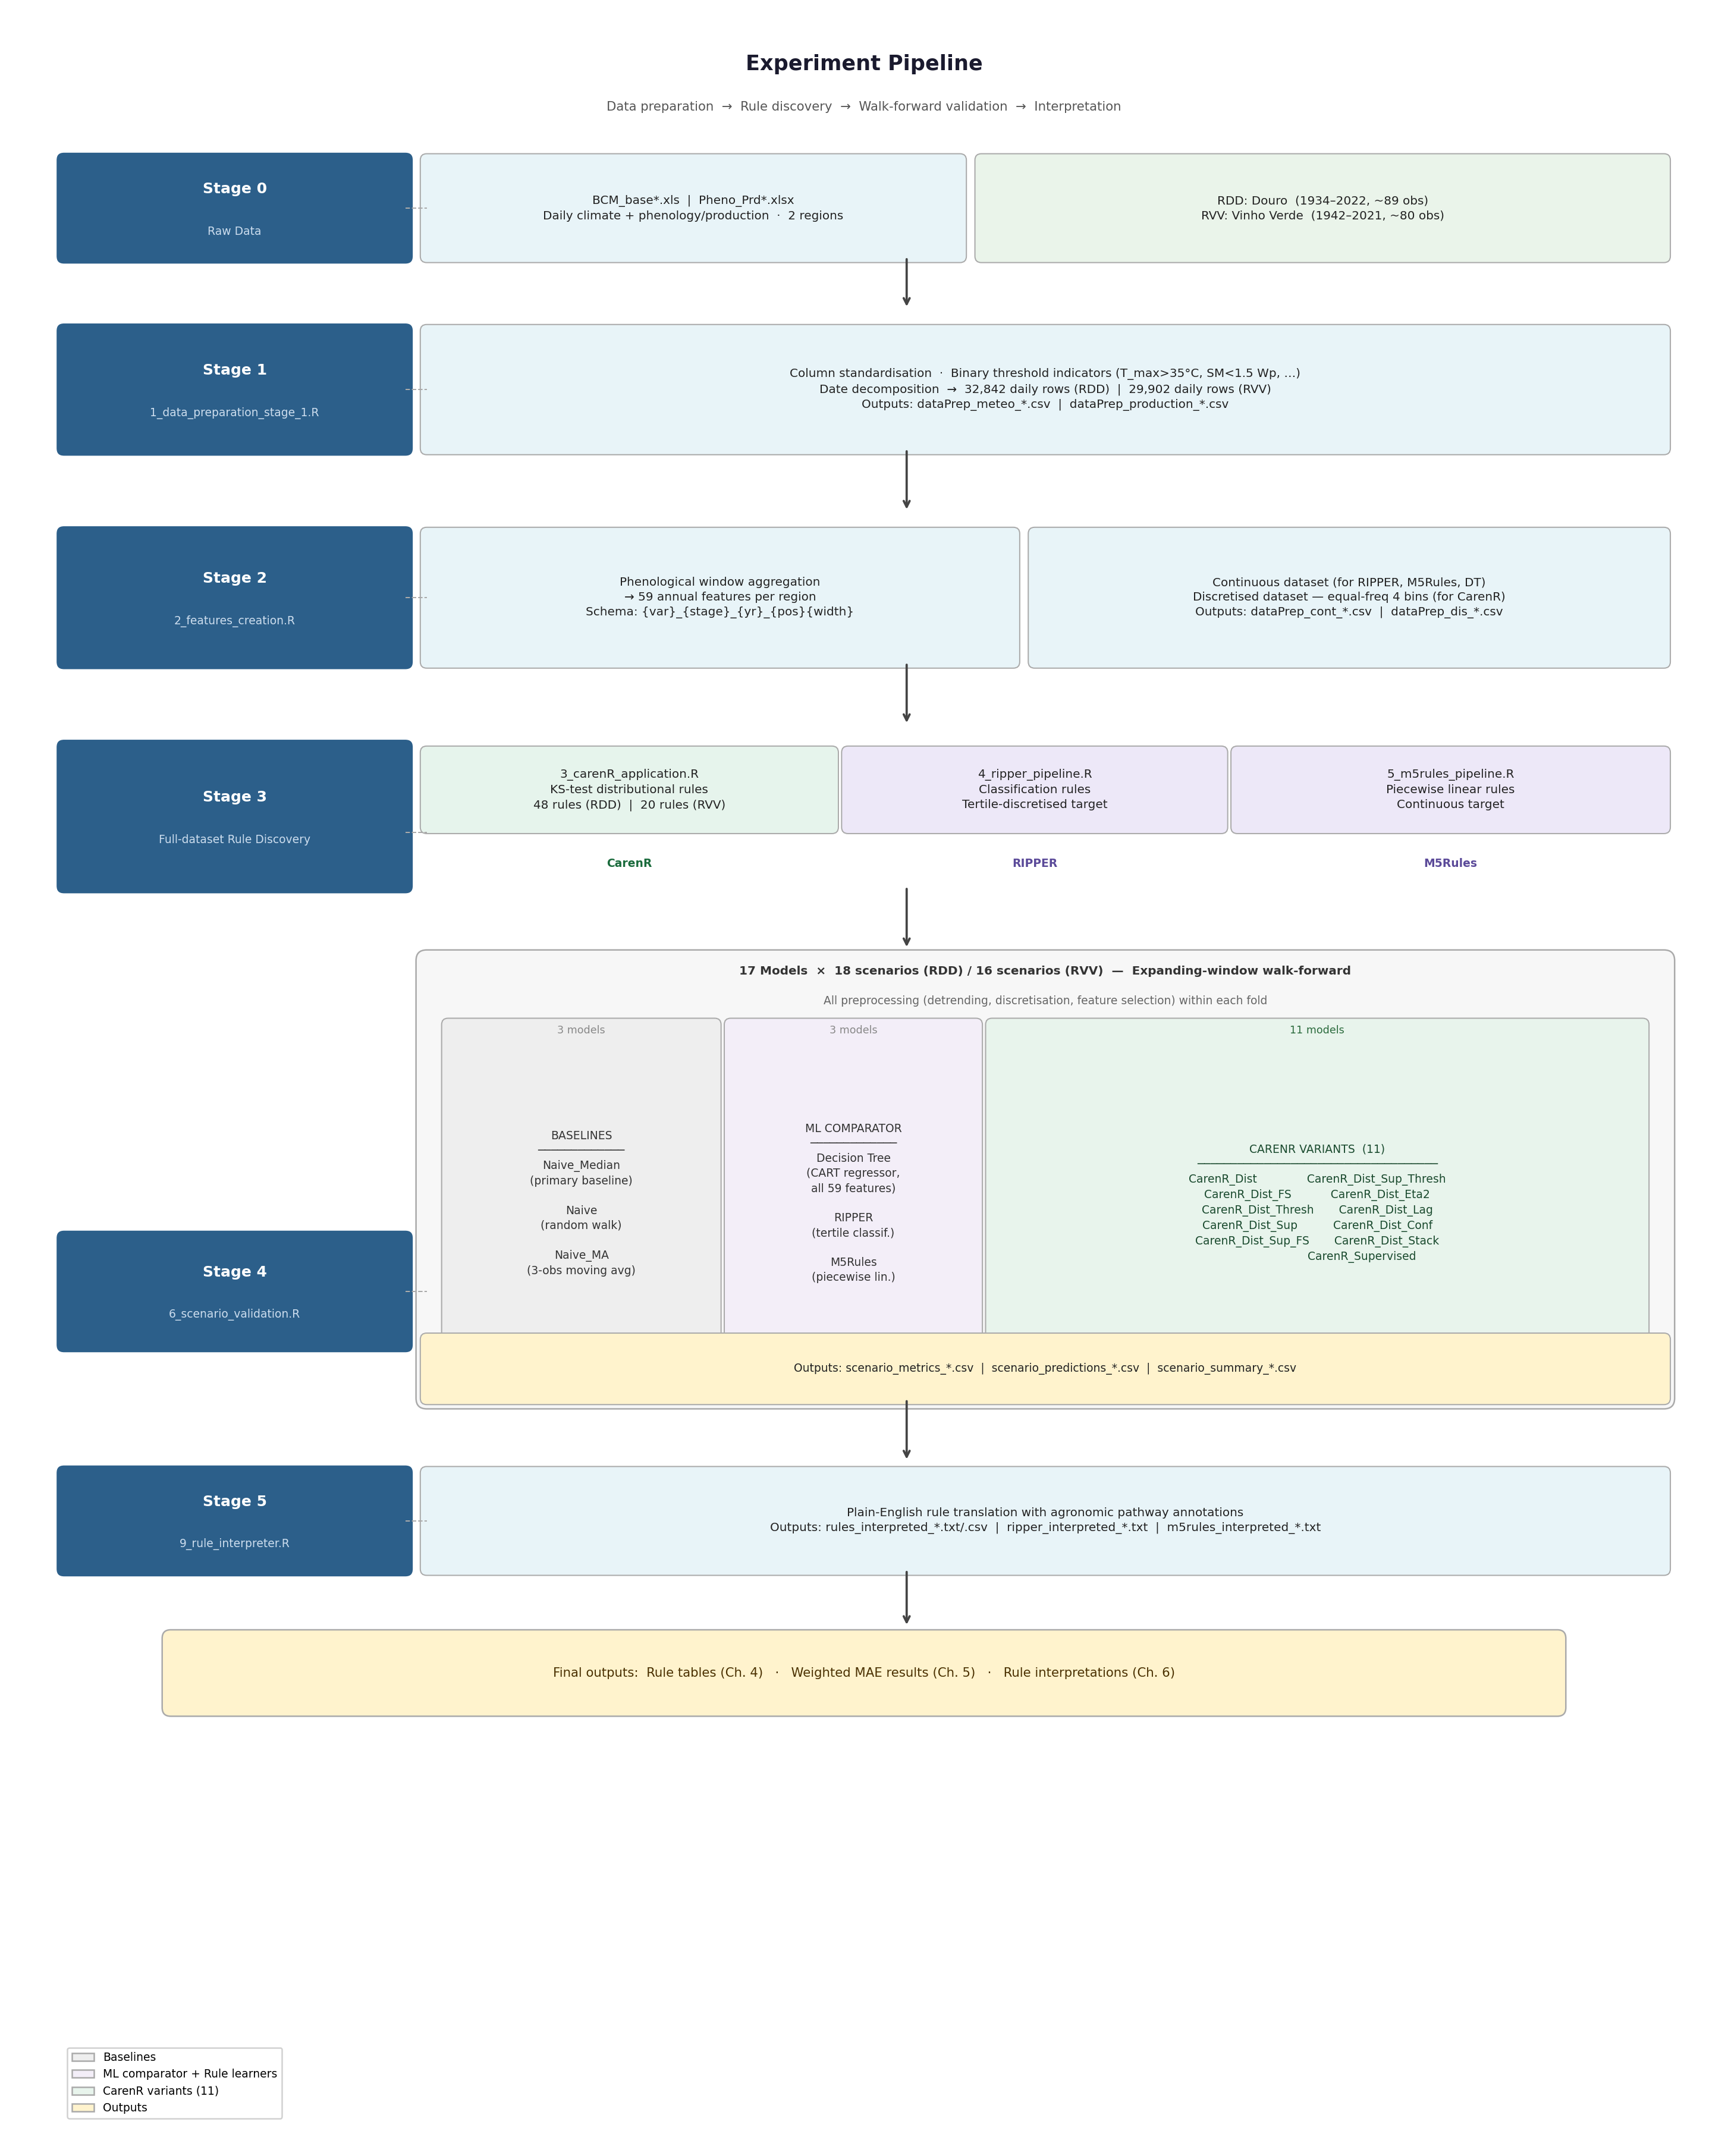
\includegraphics[width=\textwidth]{figures/fig_ch3_pipeline.png}
  \caption{Experiment pipeline: data preparation, rule discovery (CarenR, RIPPER, M5Rules), and walk-forward validation.}
  \label{fig:ch3_pipeline}
\end{figure}

Table~\ref{tab:ch3d_6} breaks the pipeline into its five numbered stages. Table~\ref{tab:ch3d_7} lists the fixed configuration parameters stored in \texttt{utils/config.R}.

\begin{table}[htbp]
  \centering
  \caption{Complete data pipeline from raw sources to final outputs.}\label{tab:ch3d_6}
  \small
  \begin{adjustbox}{max width=\textwidth}
    \begin{tabularx}{\textwidth}{p{1.5cm}|p{2.4cm}|p{2.2cm}|p{2.4cm}|X}
  \toprule
  Stage & Script & Input & Output & Key transformation \\
  \midrule
  0: Raw data & (external) & BCM\_base*.xls
Pheno\_Prd*.xlsx & Raw Excel files & Daily climate + annual phenology/production from field stations and STICS model \\
  1: Daily prep & 1\_data\_preparation\_stage\_1.R & Raw Excel files & dataPrep\_meteo\_*.csv
dataPrep\_production\_*.csv & Column standardisation, binary threshold indicators (Tmax>35, Sm<1.5Wp etc.), date decomposition. 32,842 rows (RDD), 29,902 rows (RVV). \\
  2: Feature engineering & 2\_features\_creation.R & dataPrep\_meteo\_*.csv
dataPrep\_production\_*.csv & dataPrep\_cont\_dataset\_*.csv
dataPrep\_dis\_rule\_dataset\_*.csv & Phenological window aggregation $\rightarrow$ 59 annual features per region. Equal-frequency discretisation (4 bins) for CarenR. 89 rows (RDD), 80 rows (RVV). \\
  3: Rule discovery & 3\_carenR\_\_application.R
4\_ripper\_pipeline.R
5\_m5rules\_pipeline.R & dataPrep\_*\_dataset\_*.csv & RulesTemp\_*\_linear.csv
ripper\_rules\_*.txt
m5rules\_rules\_*.txt & Full-dataset rule induction for all three algorithms. CarenR: 48 rules (RDD), 20 rules (RVV). \\
  4: Walk-forward validation & 6\_scenario\_validation.R & dataPrep\_cont\_dataset\_*.csv & scenario\_metrics\_*.csv
scenario\_predictions\_*.csv
scenario\_summary\_*.csv & 17-model $\times$ 18/16 scenario expanding-window evaluation. All preprocessing within fold. \\
  5: Rule interpretation & 9\_rule\_interpreter.R & RulesTemp\_*.csv
ripper\_rules\_*.txt
m5rules\_rules\_*.txt & rules\_interpreted\_*.txt/.csv
ripper\_interpreted\_*.txt
m5rules\_interpreted\_*.txt & Translation of raw rule outputs to plain-English descriptions with agronomic pathway annotations. \\
  \bottomrule
\end{tabularx}
  \end{adjustbox}
\end{table}

\begin{table}[htbp]
  \centering
  \caption{Fixed configuration parameters for CarenR and the walk-forward protocol.}\label{tab:ch3d_7}
  \small
  \begin{adjustbox}{max width=\textwidth}
    \begin{tabularx}{\textwidth}{l|l|X}
  \toprule
  Parameter & Value & Location in code \\
  \midrule
  Detrending method & Linear (OLS) & config.R: detrend\_method \\
  CarenR support threshold & 20\% ($s_i$ $\geq$ 0.20) & 6\_scenario\_validation.R: carenr\_min\_sup \\
  Significance threshold & p $\leq$ 0.10 & config.R: alpha\_threshold \\
  Minimum training fraction & 80\% & config.R: min\_train\_frac \\
  Feature selection strategy & Per variant ($\eta$$^2$, Pearson, or support-filtered) & config.R: fs\_strategy \\
  \bottomrule
\end{tabularx}
  \end{adjustbox}
\end{table}
